\section{Methodology}
The ODE system is solved using ode15s in Matlab with relative and absolute tolerances of $10^{-4}$.
\subsection{QoIs}
We analyse 3 quantities of interest (QoIs) with respect to two different stimulations, a 10 second square stimulation pulse and a 16 second stimulus used in lab experiments. They are displayed in Figure~\ref{input_stimuli}.
\begin{figure}[h]
\centering
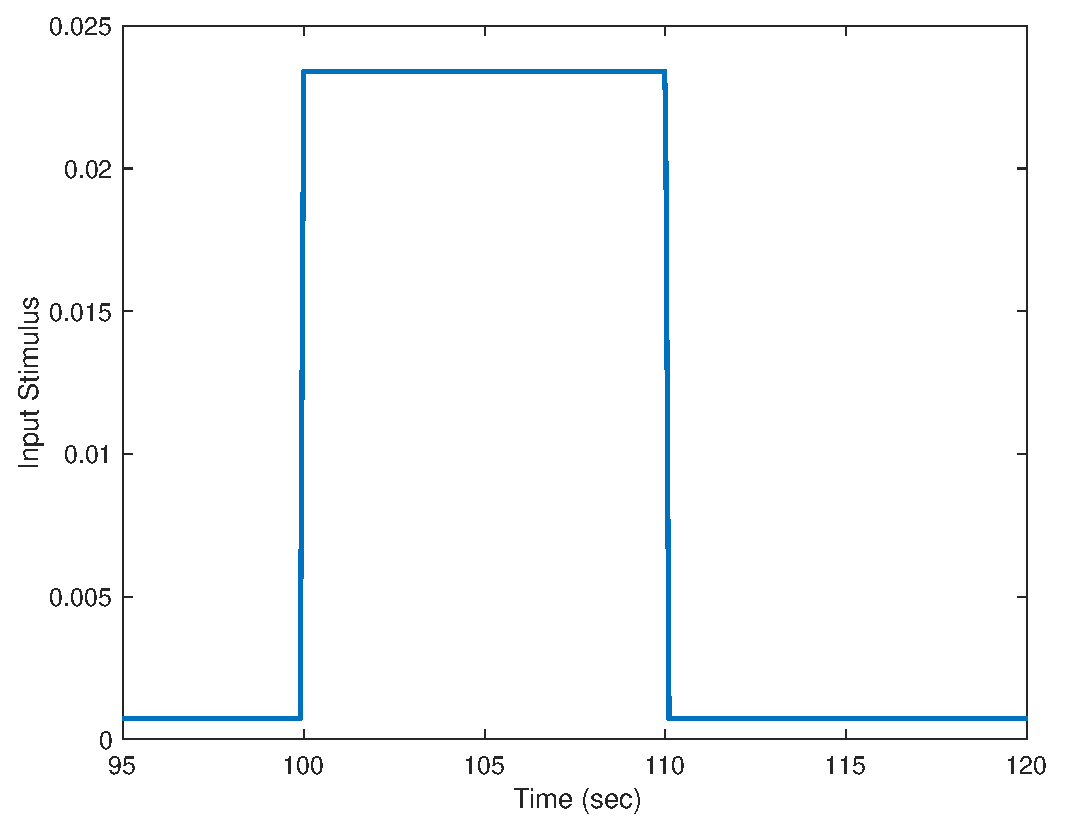
\includegraphics[width=.4 \textwidth]{Figures/Rectangular_Stimulus.eps}
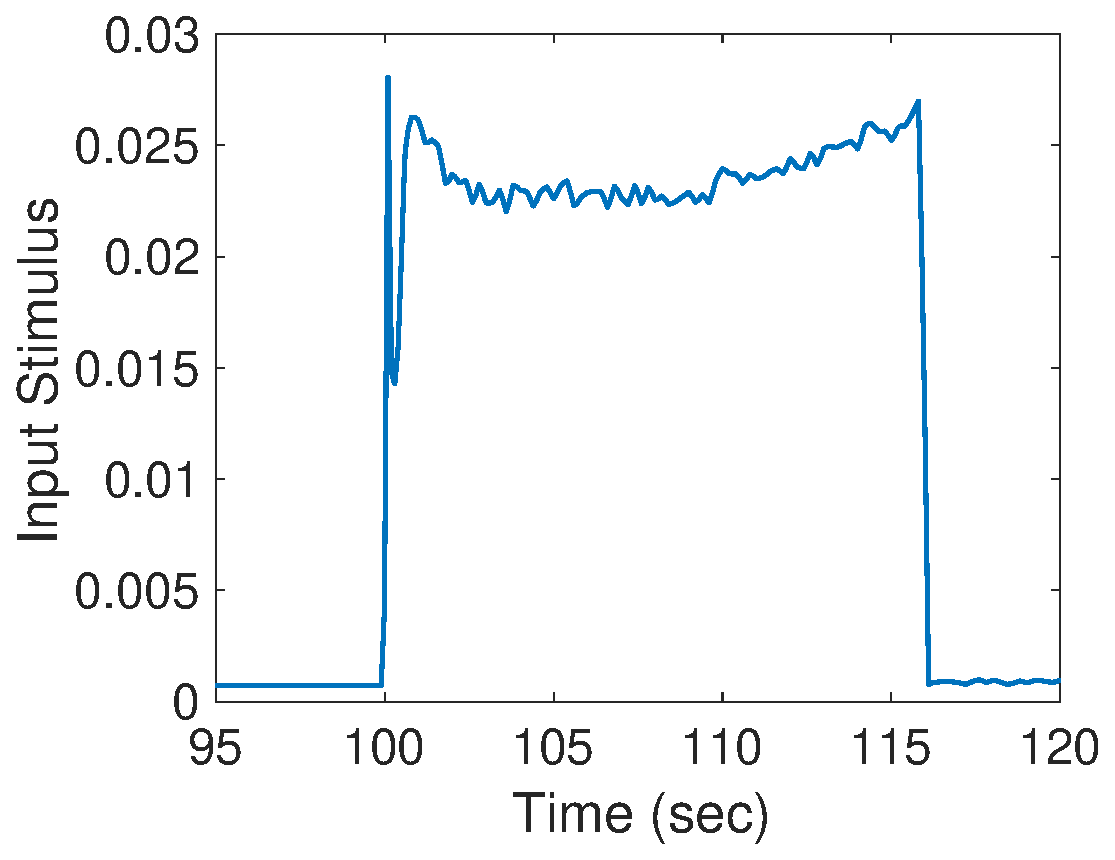
\includegraphics[width=.4 \textwidth]{Figures/Experimental_Stimulus.eps}
\caption{Left: rectangular pulse input stimulus; right: stimulus used in lab experiments.}
\label{input_stimuli}
\end{figure}
 Assuming the stimulation occurs for $t_1\le t \le t_2$, the QoIs are defined as follows.
\begin{enumerate}
\item ECS potassium has a distinct effect on the flux into the Neuron. Hence we look at the average.
\begin{eqnarray}
%[K^+]_{max,ECS} \label{K_ECS_Max} \\
 \frac{1}{t_2-t_1}\int_{t_1}^{t_2}[K^+]_{ECS}(s)ds \label{K_ECS_Mean}
\end{eqnarray}

\item As a representation of the volumetric flow rate in the cerebral tissue
\begin{equation}
\frac{1}{t_2-t_1}\int_{t_1}^{t_2}\left(\frac{R(s)}{R_0}\right)^4ds \label{vol_flow}
\end{equation}
 
%\item ECS potassium has a distinct effect on the flux into the astrocyte. Hence we look at the average and the maximum.
%\begin{eqnarray}
%[K^+]_{max,AC} \label{K_AC_Max} \\
%\frac{1}{t_2-t_1}\int_{t_1}^{t_2}[K^+]_{AC}(s)ds \label{K_AC_Mean}
%\end{eqnarray}
\item The combined concentration of the actin myosin complex, both phosphorylated and unphosphorylated, determines the effect stress due to the contraction for the smooth muscle cell. 
\begin{eqnarray}
[AM+AM_p]_{min} \label{AM_AMp_Min}
\end{eqnarray}

%\item The phase lag between neuronal stimulation and the radius changed effects a number of markers. Notably the BOLD signal, hence we choose to investigate
% the time, $\tau$, to min value of $AM_p$
% \begin{eqnarray}
% \tau = t_{min}-t_1 \label{AMp_Time_to_Min}
% \end{eqnarray}
\end{enumerate}

In addition, we consider the average concentration of AC potassium. It exhibits very small variation with respect to the parameters so we do not report any additional results for this QoI.

\subsection{Surrogate models and Sobol' indices}
There are a plurality of methods which may be used to analyse the sensitivity of a QoI to uncertain parameters. The large parameter dimension and computational cost of model evaluations prohibit many commonly used methods. A linear regression model of the form
\begin{eqnarray*}
\beta_0 + \sum\limits_{k=1}^{160} \beta_k \theta_k
\end{eqnarray*}
is fit to sample data (collected by running the model for various parameter samples) and the sensitivity of the linear model with respect to $\theta_k$ is defined as
\begin{eqnarray*}
L_k = \frac{\vert \beta_k \vert}{\sum\limits_{j=1}^{160} \vert \beta_j \vert}, \qquad k=1,2,\dots,160.
\end{eqnarray*}

In order to fit a nonlinear surrogate model, we reduce the parameter space to only the $\theta_k$'s such that $L_k>0.01$. Then a sparse Polynomial Chaos (PC) surrogate is fit using the sample data with the parameters $\{\theta_{k_i}\}_{i=1}^r$, where $L_{k_i}>0.01$, $i=1,2,\dots,r$. In Section~\ref{sec:results}, this reduction yields around $15-20$ parameters instead of the original 160. The PC surrogate is fit using the metamodel type \textit{PCE} in the UQLab \cite{uqlab}. The total Sobol' indices \cite{saltellitotalindex} of the PC surrogate are computed to yield a quantitative measure of importance for each $\theta_{k_i}$, $i=1,2,\dots,r$.

This procedure of 
\begin{enumerate}
\item[(i)] reducing dimension with linear regression,
\item[(ii)] fitting a Polynomial Chaos surrogate using the smaller set of parameters,
\item[(iii)] computing total Sobol' indices of the Polynomial Chaos surrogate,
\end{enumerate}
is used for each QoI considered in this article. All surrogate models are validated using 10-fold cross validation.
